\section{Action}\label{sec:action}


The D7-brane action \eqref{eq:DbraneAction} for our configuration \eqref{eq:ansatz} can be written as:
\begin{align} \label{eq:ActionWithTheta'}
 S  = & -T_7 \int_\mathcal{M} d^8\xi \, e^{-P[\Phi] } v_x^4 v_c v_1 v_2^2 \sqrt{1+\frac{v_\theta^2}{v_c^2}\theta'(c)^2}  \nonumber \\
      & + T_7\int _\mathcal{M} P[C_{(8)}],
\end{align}
or more explicitly, using the solution \eqref{eq:susyConditionTheta}, as:
\begin{align}\label{eq:ActionWithTheta}
 S = & -T_7 \int_\mathcal{M} d^8\xi \, \dfrac{c A(c) \cos^3\theta (c) \sqrt{X_1(c, \theta(c))}}{\left(c^2-1\right)^3} \sqrt{1+ c A(c) \tan^2\theta(c)} \nonumber \\
     & +T_7\int _\mathcal{M} d^8\xi \, \dfrac{A(c)^2 \cos^4\theta(c)}{4 \left(c^2-1\right)^2}.
\end{align}
The explicit form of the Wess-Zumino term is calculated below.

\subsection{Wess-Zumino term}
The $P[C_{(8)}]$ term was deemed vanishing in \cite{Albash:2011nw} and \cite{Evans:2005ti}. Their argument did not consider the dilaton factor in the string frame that affects the Hodge star operation while deriving $C_{(8)}$, which in our scenario is
\begin{equation}
 dC_{(8)} = \ast dC_{(0)}.
\end{equation}
The dilaton term from the string frame effectively cancels the factor that vanishes at $\phi_0$, leading to a finite value for the pullback of this potential. We decided to compute it explicitly, and the full result is given in the appendix \ref{sec:backgroundFields}. We can quickly see that it is non-zero for our ansatz for $\phi$ in \eqref{eq:ansatz}. However, $P[C_{(8)}]$ term can be much simpler, as we will see now. First, we can show that:
\begin{equation}\label{eq:C8id}
 [d C_{(8)}]_{\phi_0} = d [C_{(8)}]_{\phi_0}.
\end{equation}
The left-hand-side is simply
\begin{equation}
 [d C_{(8)}]_{\phi_0}  = \dfrac{A^2 \sin\theta \cos^3(\theta)}{\left(c^2-1\right)^2} 
\sigma_1 \wedge \sigma_2 \wedge \sigma_3 \wedge dc  \wedge dx_0 \wedge dx_1 \wedge dx_2 \wedge dx_3 \wedge d\theta,
\end{equation}
and, via \eqref{eq:C8id}, we can integrate the above expression over $\theta$ and obtain:
\begin{equation}
[C_{(8)}]_{\phi_0} = \dfrac{A^2 \cos^4\theta}{4 \left(c^2-1\right)^2} \sigma_1 \wedge \sigma_2 \wedge \sigma_3 \wedge dc \wedge dx_0 \wedge dx_1 \wedge dx_2 \wedge dx_3.
\end{equation}
The full pullback is obtained by just replacing $\theta$ by $\theta(c)$.




%%%%%%%%%%%%%%%%%%%%%%%%%%%%%%%%%%%%%%%%%%%%%%%%%%%%%%%%%%%%%%%%%%%%%%%%%%%%%%%%%%%%%%%%%%%%%%%%%

\subsection{Equation of motion}

As a consistency check for our results, the equation of motion from the action \eqref{eq:ActionWithTheta'} is fulfilled with the solution \eqref{eq:susyConditionTheta}. In particular, 
\begin{align}\label{eq:eom}
-\left.EL[\mathcal{L}_{DBI}]\right|_\text{solution} = EL[\mathcal{L}_{WZ}] = \dfrac{A^2 \sin\theta \cos^3(\theta)}{\left(c^2-1\right)^2},
\end{align}
where $EL[\cdot]$ is the Euler-Lagrange operator:
\begin{equation}
 EL[\mathcal{L}] = 
 \left(\dfrac{\pd }{\pd \theta(c)} -\dfrac{\pd }{\pd c}  \dfrac{\pd }{\pd \theta'(c)} \right) \mathcal{L}.
\end{equation}
Therefore, \eqref{eq:eom} is another proof for the non-vanishing WZ term.



\subsection{Holographic renormalization}
The fully explicit on-shell action evaluated at the solution \eqref{eq:susyConditionSolution} is:
\begin{align}\label{eq:ActionAtSolution}
 S_\text{reg} = -T_7 V \int_{1 + \epsilon^2/2}^{c_\text{max}} d c \, 
 &\left[-\frac{c A(c)}{\left(c^2-1\right)^3} -\frac{A(c)^2}{4 \left(c^2-1\right)^2} \right. \nonumber\\
 &-\frac{L^2 A(c) \left(\left(c^2+1\right) A(c)-4 c\right)}{2 \left(c^2-1\right)^2} \nonumber\\
 &+\left.\frac{L^4 A(c) \left(3 c^2 A(c)+A(c)-4 c\right)}{4 \left(c^2-1\right)}\right],
\end{align}
where $c_\text{max}$ is the upper bound shown in \eqref{eq:susyConditionSolution}, and $V$ denotes the volume of the 4-dimensional Minkowski space times the 3-sphere. Notice that the action is divergent near the boundary, thus, we regularized it by adding a regulator $\epsilon>0$ in the lower integration limit. Let us also introduce the following notation regarding the integration limits:
\begin{equation}
  S_\text{reg} \equiv S_\text{IR}-S_\text{UV}.
\end{equation}


From the exact integrations in the appendix \ref{sec:integrate-action}, we can identify the divergent terms:
\begin{align} \label{eq:Sdiv}
 S_\text{div} = T_7 V 
        \left[ \frac{1}{4 \epsilon ^4} +\frac{1+\log \left(\epsilon/2\right)}{2 \epsilon ^2}-\frac{L^2}{2 \epsilon ^2}-\frac{ \log ^2\left(\epsilon/2\right)}{4}+\frac{\log (\epsilon )}{8} \right],
\end{align}
which come from the $L^0$ and $L^2$ terms of \eqref{eq:ActionAtSolution}. 

In holographic renormalization, the counterterms must be covariant and local on the regulator hypersurface. They do not only subtract the divergences, but also finite terms from both IR and UV regions, such that the final action vanishes, as required by supersymmetry. For general asymptotic AdS spaces and for the D7-brane in particular, the counterterms are derived in \cite{Karch:2005ms} (we do not copy the ones with curvature below):
\begin{align} \label{eq:Ls}
& L_{1}=-\frac{1}{4} \sqrt{\gamma} \nonumber\\
& L_{4}=\frac{1}{2} \sqrt{\gamma} \theta(\epsilon)^2 \nonumber\\
& L_{f}= -\frac{5}{12}\sqrt{\gamma} \theta(\epsilon)^4,
\end{align}
where $\gamma$ here denotes the determinant of the regulator hypersurface metric. 
However, for our case, these counterterms do not apply. Our geometry is seemingly not covered by this general study, due to the logarithmic divergence appearing already at the next-to-leading order $\epsilon$-expansion for the metric, coming from $A(c)$. The explanation is that the 10-dimensional Pilch-Warner background is uplifted from the 5-dimensional supergravity solution, and indeed the logarithmic divergence mentioned comes from fields in the 5-dimensional theory, not from the 5-dimensional metric; see \cite{Bobev:2013cja}. If we were to find covariant counterterms, these would be written in terms of these lower dimensional fields too.


Let us be concerned about the counterterms that cancel exactly $S_\text{div}$, for now. We propose:
\begin{equation}\label{eq:counterterms}
 S_\text{CT, UV} =  T_7 V \left[ 
  \frac{1}{4} \sqrt{\gamma} f(\epsilon)
   -\frac{1}{2} \sqrt{\gamma} \theta (\epsilon)^2 + \frac{1}{6} \sqrt{\gamma} \theta (\epsilon)^4
   \right],
\end{equation}
where the scalar field expansion is found in \eqref{eq:thetaExpanded}, and we defined
\begin{align}
 \sqrt{\gamma} &= \frac{1}{\epsilon^4}-\frac{1}{2 \epsilon ^2},\\
 f(\epsilon) &= 1 + 12 \alpha(\epsilon) + 6 \,(1 + 8 \alpha(\epsilon )) \chi(\epsilon ) ^2+14 \chi(\epsilon )^4, \label{eq:f}
\end{align}
where $\alpha(\epsilon)$ and $\chi(\epsilon)$ are scalar fields living in the 5-dimensional supergravity; we follow the notation in \cite{Albash:2011nw}, and our $A$ is their $\rho^6$.
The expression $f(\epsilon)$ is obtained from the numerator of \eqref{eq:I0} with the replacements 
\begin{align}
c &= \cosh(2 \, \chi) \approx 1 + 2 \chi ^2 + \frac{2}{3}\chi ^4,\\
A &= \exp{(6 \, \alpha)}\approx 1 + 6 \alpha + 18 \alpha ^2. 
\end{align}
From $c = 1 + \epsilon^2/2$ and the asymptotic expansions of $A$ in \eqref{eq:expandA}, we know that $\chi \propto \epsilon$ and $\alpha \propto \epsilon^2$ at the leading order. Then, for $f(\epsilon)$ we keep only the terms up to order $\epsilon^4$.  

In \eqref{eq:counterterms}, there is also a finite counterterm in terms of the quartic power of the scalar field. This is there to cancel the finite term introduced by the counterterm quadratic in the scalar field. 

The IR contribution to the action, $S_\text{IR}$, obtained by evaluating the integrals in \ref{sec:integrate-action} at $c=\sqrt{1+L^{-2}}$, are highly non-trivial functions of $L$, see figure \ref{fig:SIR}.
We are not able to find covariant counterterms to cancel them, and think it is not possible. 
As for the supergravity side, this is a finite term ambiguity in the renormalization scheme. 
However, from the field theory point of view, if we cannot write the counterterm in the covariant form, it would imply a non-vanishing action, and hence, a non-vanishing chiral condensate. 
It is known for $\mathcal{N}=1$ SYM theory that the chiral symmetry spontaneously breaks; see for example \cite{Bergner:2014saa}. Since our field theory also has one copy of supersymmetry, it is then possible that the condensate could be non-zero. We will leave a more detailed study of the dual field theory interpretation for future works.

\begin{figure}[t]
\begin{center}
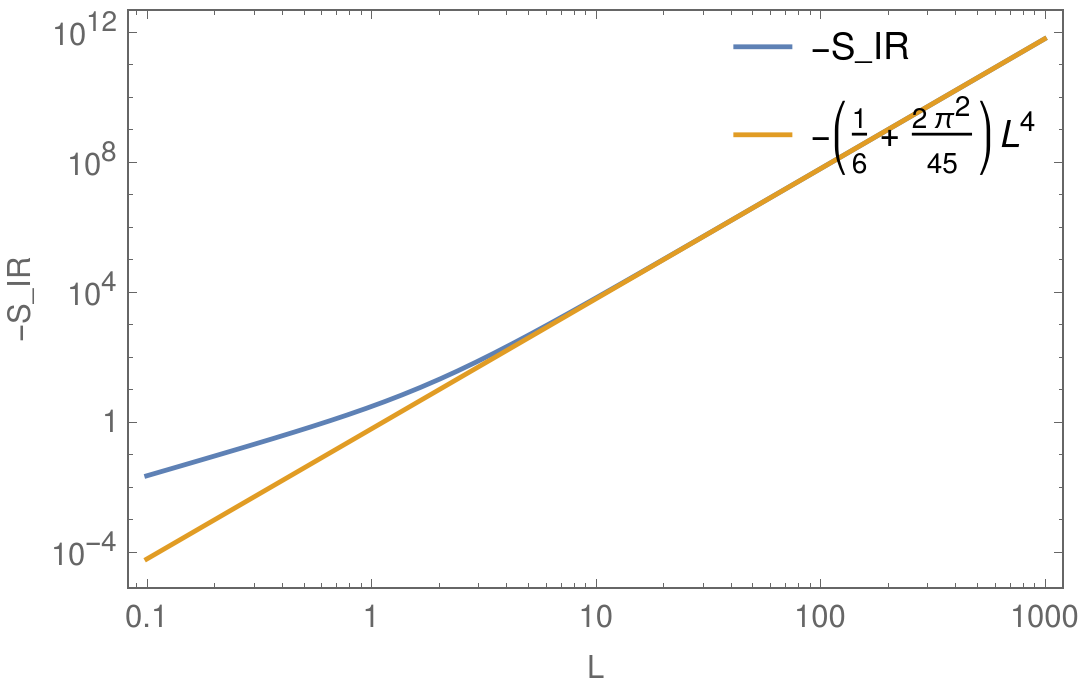
\includegraphics[width=0.6\textwidth]{pictures/SIR.png}
\end{center}
\caption{\label{fig:SIR} This is a double logarithmic plot of the negative of the IR contribution to the action, $S_\text{IR}$, and its limiting behavior at large $L$.}
\end{figure}

As our last consistency check of our findings, let us study the large $L$ limit in the subsection below. 

\subsubsection{Large L}
As we discussed in \ref{sec:solution}, our embedding matches with the one in the $AdS_5 \times S^5$ background in the near-boundary expansion and at the large $L$ limit. 
The large $L$-expansion of the action is found in \ref{sec:IRlimit}. 
The finite terms from $S_\text{UV}$ are shown in \ref{sec:UVlimit}.
Finally, at the leading order in $L$, the total finite term is:
\begin{equation} 
S_\text{IR}-S_\text{UV}+S_\text{CT,UV} = - T_7 V \frac{1}{4} L^4 +O(L^2 \log L)
\end{equation}
Taking this term into account, the full counterterm action at the large $L$ limit is:
\begin{equation}
 S_\text{CT} =  T_7 V \left[ 
  \frac{1}{4} \sqrt{\gamma} f(\epsilon)
   -\frac{1}{2} \sqrt{\gamma} \theta (\epsilon)^2 + \frac{5}{12} \sqrt{\gamma} \theta (\epsilon)^4
   \right], \quad (L\gg 1).
\end{equation}
This indeed matches with the general counterterms \eqref{eq:Ls} if we set the fields in \eqref{eq:f} to zero.

The renormalized action, defined as
\begin{equation}
 S_\text{ren} = \lim_{\epsilon\rightarrow 0} (S_\text{reg}-S_\text{CT}),
\end{equation}
is hence exactly zero at the large $L$ limit. Consequently, the chiral condensate, sourced by $L$, also vanishes:
\begin{equation} 
\langle O \rangle = \frac{\delta S_\text{ren}}{\delta L} = 0. 
\end{equation}




 




